\renewcommand{\leveltopI}{-15cm + \leveltop}
\renewcommand{\leveltopII}{-15cm + \leveltopI}
\renewcommand{\leveltopIII}{-15cm + \leveltopII}
\renewcommand{\leveltopIIII}{-15cm + \leveltopIII}
\renewcommand{\leveltopIIIII}{-15cm + \leveltopIIII}
\renewcommand{\leveltopIIIIII}{-15cm + \leveltopIIIII}
\renewcommand{\leveltopIIIIIII}{-15cm + \leveltopIIIIII}
\renewcommand{\leveltopIIIIIIII}{-15cm + \leveltopIIIIIII}
\renewcommand{\leveltopIIIIIIIII}{-15cm + \leveltopIIIIIIII}
\renewcommand{\leveltopIIIIIIIIII}{-15cm + \leveltopIIIIIIIII}
\renewcommand{\leveltopIIIIIIIIIII}{-15cm + \leveltopIIIIIIIIII}
\begin{tikzpicture}[scale=.2, anchor=south]
  \begin{scope}[yshift=\leveltopI cm]
    \matrix (line1) [column sep=1cm] {
      \node[draw=black, rectangle split,  rectangle split parts=3] (sn0x104f980){
        \begin{tikzpicture}[scale=.2]
          \node[circle, scale=0.75, fill] (tid0) at (3.75,1.5){};
          \node[circle, scale=0.75, fill] (tid1) at (2.25,3){};
          \node[circle, scale=0.75, fill] (tid3) at (0.75,4.5){};
          \node[circle, scale=0.75, fill] (tid7) at (0.75,6){};
          \draw[](tid3) -- (tid7);
          \node[circle, scale=0.75, fill] (tid4) at (2.25,4.5){};
          \node[circle, scale=0.75, fill] (tid5) at (3.75,4.5){};
          \draw[](tid1) -- (tid3);
          \draw[](tid1) -- (tid4);
          \draw[](tid1) -- (tid5);
          \node[circle, scale=0.75, fill] (tid2) at (6,3){};
          \node[circle, scale=0.75, fill] (tid6) at (6,4.5){};
          \node[circle, scale=0.75, fill] (tid8) at (5.25,6){};
          \node[circle, scale=0.75, fill, red] (tid10) at (5.25,7.5){};
          \draw[](tid8) -- (tid10);
          \node[circle, scale=0.75, fill, red] (tid9) at (6.75,6){};
          \draw[](tid6) -- (tid8);
          \draw[](tid6) -- (tid9);
          \draw[](tid2) -- (tid6);
          \draw[](tid0) -- (tid1);
          \draw[](tid0) -- (tid2);
        \end{tikzpicture}
        \nodepart{two}
        \footnotesize{6.82812}
        \nodepart{three}
        \footnotesize{$50\:25\:25$}
      };
      & 
      \\
    };
  \end{scope}
  \begin{scope}[yshift=\leveltopII cm]
    \matrix (line2) [column sep=1cm] {
      \node[draw=black, rectangle split,  rectangle split parts=3] (sn0x1050190){
        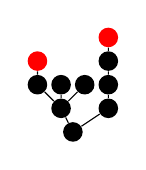
\begin{tikzpicture}[scale=.2]
          \node[circle, scale=0.75, fill] (tid0) at (3,1.5){};
          \node[circle, scale=0.75, fill] (tid1) at (2.25,3){};
          \node[circle, scale=0.75, fill] (tid3) at (0.75,4.5){};
          \node[circle, scale=0.75, fill, red] (tid7) at (0.75,6){};
          \draw[](tid3) -- (tid7);
          \node[circle, scale=0.75, fill] (tid4) at (2.25,4.5){};
          \node[circle, scale=0.75, fill] (tid5) at (3.75,4.5){};
          \draw[](tid1) -- (tid3);
          \draw[](tid1) -- (tid4);
          \draw[](tid1) -- (tid5);
          \node[circle, scale=0.75, fill] (tid2) at (5.25,3){};
          \node[circle, scale=0.75, fill] (tid6) at (5.25,4.5){};
          \node[circle, scale=0.75, fill] (tid8) at (5.25,6){};
          \node[circle, scale=0.75, fill, red] (tid9) at (5.25,7.5){};
          \draw[](tid8) -- (tid9);
          \draw[](tid6) -- (tid8);
          \draw[](tid2) -- (tid6);
          \draw[](tid0) -- (tid1);
          \draw[](tid0) -- (tid2);
        \end{tikzpicture}
        \nodepart{two}
        \footnotesize{6.35938}
        \nodepart{three}
        \footnotesize{$50\:50$}
      };
      & 
      \node[draw=black, rectangle split,  rectangle split parts=3] (sn0x104cb60){
        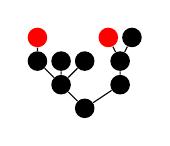
\begin{tikzpicture}[scale=.2]
          \node[circle, scale=0.75, fill] (tid0) at (3.75,1.5){};
          \node[circle, scale=0.75, fill] (tid1) at (2.25,3){};
          \node[circle, scale=0.75, fill] (tid3) at (0.75,4.5){};
          \node[circle, scale=0.75, fill, red] (tid7) at (0.75,6){};
          \draw[](tid3) -- (tid7);
          \node[circle, scale=0.75, fill] (tid4) at (2.25,4.5){};
          \node[circle, scale=0.75, fill] (tid5) at (3.75,4.5){};
          \draw[](tid1) -- (tid3);
          \draw[](tid1) -- (tid4);
          \draw[](tid1) -- (tid5);
          \node[circle, scale=0.75, fill] (tid2) at (6,3){};
          \node[circle, scale=0.75, fill] (tid6) at (6,4.5){};
          \node[circle, scale=0.75, fill, red] (tid8) at (5.25,6){};
          \node[circle, scale=0.75, fill] (tid9) at (6.75,6){};
          \draw[](tid6) -- (tid8);
          \draw[](tid6) -- (tid9);
          \draw[](tid2) -- (tid6);
          \draw[](tid0) -- (tid1);
          \draw[](tid0) -- (tid2);
        \end{tikzpicture}
        \nodepart{two}
        \footnotesize{6.29688}
        \nodepart{three}
        \footnotesize{$50\:50$}
      };
      & 
      \node[draw=black, rectangle split,  rectangle split parts=3] (sn0x104dd20){
        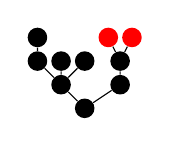
\begin{tikzpicture}[scale=.2]
          \node[circle, scale=0.75, fill] (tid0) at (3.75,1.5){};
          \node[circle, scale=0.75, fill] (tid1) at (2.25,3){};
          \node[circle, scale=0.75, fill] (tid3) at (0.75,4.5){};
          \node[circle, scale=0.75, fill] (tid7) at (0.75,6){};
          \draw[](tid3) -- (tid7);
          \node[circle, scale=0.75, fill] (tid4) at (2.25,4.5){};
          \node[circle, scale=0.75, fill] (tid5) at (3.75,4.5){};
          \draw[](tid1) -- (tid3);
          \draw[](tid1) -- (tid4);
          \draw[](tid1) -- (tid5);
          \node[circle, scale=0.75, fill] (tid2) at (6,3){};
          \node[circle, scale=0.75, fill] (tid6) at (6,4.5){};
          \node[circle, scale=0.75, fill, red] (tid8) at (5.25,6){};
          \node[circle, scale=0.75, fill, red] (tid9) at (6.75,6){};
          \draw[](tid6) -- (tid8);
          \draw[](tid6) -- (tid9);
          \draw[](tid2) -- (tid6);
          \draw[](tid0) -- (tid1);
          \draw[](tid0) -- (tid2);
        \end{tikzpicture}
        \nodepart{two}
        \footnotesize{6.29688}
        \nodepart{three}
        \footnotesize{$1$}
      };
      & 
      \\
    };
  \end{scope}
  \begin{scope}[yshift=\leveltopIII cm]
    \matrix (line3) [column sep=1cm] {
      \node[draw=black, rectangle split,  rectangle split parts=3] (sn0x10519d0){
        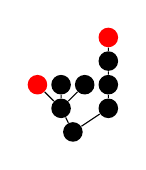
\begin{tikzpicture}[scale=.2]
          \node[circle, scale=0.75, fill] (tid0) at (3,1.5){};
          \node[circle, scale=0.75, fill] (tid1) at (2.25,3){};
          \node[circle, scale=0.75, fill, red] (tid3) at (0.75,4.5){};
          \node[circle, scale=0.75, fill] (tid4) at (2.25,4.5){};
          \node[circle, scale=0.75, fill] (tid5) at (3.75,4.5){};
          \draw[](tid1) -- (tid3);
          \draw[](tid1) -- (tid4);
          \draw[](tid1) -- (tid5);
          \node[circle, scale=0.75, fill] (tid2) at (5.25,3){};
          \node[circle, scale=0.75, fill] (tid6) at (5.25,4.5){};
          \node[circle, scale=0.75, fill] (tid7) at (5.25,6){};
          \node[circle, scale=0.75, fill, red] (tid8) at (5.25,7.5){};
          \draw[](tid7) -- (tid8);
          \draw[](tid6) -- (tid7);
          \draw[](tid2) -- (tid6);
          \draw[](tid0) -- (tid1);
          \draw[](tid0) -- (tid2);
        \end{tikzpicture}
        \nodepart{two}
        \footnotesize{5.92188}
        \nodepart{three}
        \footnotesize{$50\:50$}
      };
      & 
      \node[draw=black, rectangle split,  rectangle split parts=3] (sn0x104fbd0){
        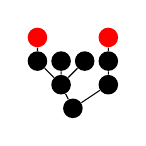
\begin{tikzpicture}[scale=.2]
          \node[circle, scale=0.75, fill] (tid0) at (3,1.5){};
          \node[circle, scale=0.75, fill] (tid1) at (2.25,3){};
          \node[circle, scale=0.75, fill] (tid3) at (0.75,4.5){};
          \node[circle, scale=0.75, fill, red] (tid7) at (0.75,6){};
          \draw[](tid3) -- (tid7);
          \node[circle, scale=0.75, fill] (tid4) at (2.25,4.5){};
          \node[circle, scale=0.75, fill] (tid5) at (3.75,4.5){};
          \draw[](tid1) -- (tid3);
          \draw[](tid1) -- (tid4);
          \draw[](tid1) -- (tid5);
          \node[circle, scale=0.75, fill] (tid2) at (5.25,3){};
          \node[circle, scale=0.75, fill] (tid6) at (5.25,4.5){};
          \node[circle, scale=0.75, fill, red] (tid8) at (5.25,6){};
          \draw[](tid6) -- (tid8);
          \draw[](tid2) -- (tid6);
          \draw[](tid0) -- (tid1);
          \draw[](tid0) -- (tid2);
        \end{tikzpicture}
        \nodepart{two}
        \footnotesize{5.79688}
        \nodepart{three}
        \footnotesize{$50\:33\:17$}
      };
      & 
      \node[draw=black, rectangle split,  rectangle split parts=3] (sn0x105a080){
        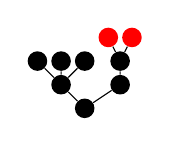
\begin{tikzpicture}[scale=.2]
          \node[circle, scale=0.75, fill] (tid0) at (3.75,1.5){};
          \node[circle, scale=0.75, fill] (tid1) at (2.25,3){};
          \node[circle, scale=0.75, fill] (tid3) at (0.75,4.5){};
          \node[circle, scale=0.75, fill] (tid4) at (2.25,4.5){};
          \node[circle, scale=0.75, fill] (tid5) at (3.75,4.5){};
          \draw[](tid1) -- (tid3);
          \draw[](tid1) -- (tid4);
          \draw[](tid1) -- (tid5);
          \node[circle, scale=0.75, fill] (tid2) at (6,3){};
          \node[circle, scale=0.75, fill] (tid6) at (6,4.5){};
          \node[circle, scale=0.75, fill, red] (tid7) at (5.25,6){};
          \node[circle, scale=0.75, fill, red] (tid8) at (6.75,6){};
          \draw[](tid6) -- (tid7);
          \draw[](tid6) -- (tid8);
          \draw[](tid2) -- (tid6);
          \draw[](tid0) -- (tid1);
          \draw[](tid0) -- (tid2);
        \end{tikzpicture}
        \nodepart{two}
        \footnotesize{5.79688}
        \nodepart{three}
        \footnotesize{$1$}
      };
      & 
      \\
    };
  \end{scope}
  \begin{scope}[yshift=\leveltopIIII cm]
    \matrix (line4) [column sep=1cm] {
      \node[draw=black, rectangle split,  rectangle split parts=3] (sn0x1052250){
        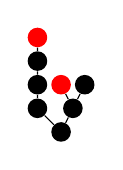
\begin{tikzpicture}[scale=.2]
          \node[circle, scale=0.75, fill] (tid0) at (2.25,1.5){};
          \node[circle, scale=0.75, fill] (tid1) at (0.75,3){};
          \node[circle, scale=0.75, fill] (tid3) at (0.75,4.5){};
          \node[circle, scale=0.75, fill] (tid6) at (0.75,6){};
          \node[circle, scale=0.75, fill, red] (tid7) at (0.75,7.5){};
          \draw[](tid6) -- (tid7);
          \draw[](tid3) -- (tid6);
          \draw[](tid1) -- (tid3);
          \node[circle, scale=0.75, fill] (tid2) at (3,3){};
          \node[circle, scale=0.75, fill, red] (tid4) at (2.25,4.5){};
          \node[circle, scale=0.75, fill] (tid5) at (3.75,4.5){};
          \draw[](tid2) -- (tid4);
          \draw[](tid2) -- (tid5);
          \draw[](tid0) -- (tid1);
          \draw[](tid0) -- (tid2);
        \end{tikzpicture}
        \nodepart{two}
        \footnotesize{5.54688}
        \nodepart{three}
        \footnotesize{$50\:50$}
      };
      & 
      \node[draw=black, rectangle split,  rectangle split parts=3] (sn0x1052960){
        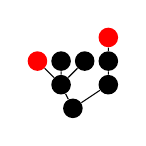
\begin{tikzpicture}[scale=.2]
          \node[circle, scale=0.75, fill] (tid0) at (3,1.5){};
          \node[circle, scale=0.75, fill] (tid1) at (2.25,3){};
          \node[circle, scale=0.75, fill, red] (tid3) at (0.75,4.5){};
          \node[circle, scale=0.75, fill] (tid4) at (2.25,4.5){};
          \node[circle, scale=0.75, fill] (tid5) at (3.75,4.5){};
          \draw[](tid1) -- (tid3);
          \draw[](tid1) -- (tid4);
          \draw[](tid1) -- (tid5);
          \node[circle, scale=0.75, fill] (tid2) at (5.25,3){};
          \node[circle, scale=0.75, fill] (tid6) at (5.25,4.5){};
          \node[circle, scale=0.75, fill, red] (tid7) at (5.25,6){};
          \draw[](tid6) -- (tid7);
          \draw[](tid2) -- (tid6);
          \draw[](tid0) -- (tid1);
          \draw[](tid0) -- (tid2);
        \end{tikzpicture}
        \nodepart{two}
        \footnotesize{5.29688}
        \nodepart{three}
        \footnotesize{$50\:33\:17$}
      };
      & 
      \node[draw=black, rectangle split,  rectangle split parts=3] (sn0x10581e0){
        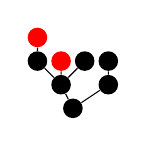
\begin{tikzpicture}[scale=.2]
          \node[circle, scale=0.75, fill] (tid0) at (3,1.5){};
          \node[circle, scale=0.75, fill] (tid1) at (2.25,3){};
          \node[circle, scale=0.75, fill] (tid3) at (0.75,4.5){};
          \node[circle, scale=0.75, fill, red] (tid7) at (0.75,6){};
          \draw[](tid3) -- (tid7);
          \node[circle, scale=0.75, fill, red] (tid4) at (2.25,4.5){};
          \node[circle, scale=0.75, fill] (tid5) at (3.75,4.5){};
          \draw[](tid1) -- (tid3);
          \draw[](tid1) -- (tid4);
          \draw[](tid1) -- (tid5);
          \node[circle, scale=0.75, fill] (tid2) at (5.25,3){};
          \node[circle, scale=0.75, fill] (tid6) at (5.25,4.5){};
          \draw[](tid2) -- (tid6);
          \draw[](tid0) -- (tid1);
          \draw[](tid0) -- (tid2);
        \end{tikzpicture}
        \nodepart{two}
        \footnotesize{5.29688}
        \nodepart{three}
        \footnotesize{$33\:17\:25\:25$}
      };
      & 
      \node[draw=black, rectangle split,  rectangle split parts=3] (sn0x1058550){
        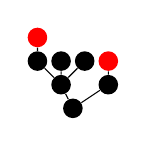
\begin{tikzpicture}[scale=.2]
          \node[circle, scale=0.75, fill] (tid0) at (3,1.5){};
          \node[circle, scale=0.75, fill] (tid1) at (2.25,3){};
          \node[circle, scale=0.75, fill] (tid3) at (0.75,4.5){};
          \node[circle, scale=0.75, fill, red] (tid7) at (0.75,6){};
          \draw[](tid3) -- (tid7);
          \node[circle, scale=0.75, fill] (tid4) at (2.25,4.5){};
          \node[circle, scale=0.75, fill] (tid5) at (3.75,4.5){};
          \draw[](tid1) -- (tid3);
          \draw[](tid1) -- (tid4);
          \draw[](tid1) -- (tid5);
          \node[circle, scale=0.75, fill] (tid2) at (5.25,3){};
          \node[circle, scale=0.75, fill, red] (tid6) at (5.25,4.5){};
          \draw[](tid2) -- (tid6);
          \draw[](tid0) -- (tid1);
          \draw[](tid0) -- (tid2);
        \end{tikzpicture}
        \nodepart{two}
        \footnotesize{5.29688}
        \nodepart{three}
        \footnotesize{$50\:50$}
      };
      & 
      \\
    };
  \end{scope}
  \begin{scope}[yshift=\leveltopIIIII cm]
    \matrix (line5) [column sep=1cm] {
      \node[draw=black, rectangle split,  rectangle split parts=3] (sn0x10525f0){
        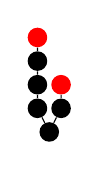
\begin{tikzpicture}[scale=.2]
          \node[circle, scale=0.75, fill] (tid0) at (1.5,1.5){};
          \node[circle, scale=0.75, fill] (tid1) at (0.75,3){};
          \node[circle, scale=0.75, fill] (tid3) at (0.75,4.5){};
          \node[circle, scale=0.75, fill] (tid5) at (0.75,6){};
          \node[circle, scale=0.75, fill, red] (tid6) at (0.75,7.5){};
          \draw[](tid5) -- (tid6);
          \draw[](tid3) -- (tid5);
          \draw[](tid1) -- (tid3);
          \node[circle, scale=0.75, fill] (tid2) at (2.25,3){};
          \node[circle, scale=0.75, fill, red] (tid4) at (2.25,4.5){};
          \draw[](tid2) -- (tid4);
          \draw[](tid0) -- (tid1);
          \draw[](tid0) -- (tid2);
        \end{tikzpicture}
        \nodepart{two}
        \footnotesize{5.25}
        \nodepart{three}
        \footnotesize{$50\:50$}
      };
      & 
      \node[draw=black, rectangle split,  rectangle split parts=3] (sn0x1053850){
        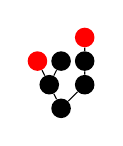
\begin{tikzpicture}[scale=.2]
          \node[circle, scale=0.75, fill] (tid0) at (2.25,1.5){};
          \node[circle, scale=0.75, fill] (tid1) at (1.5,3){};
          \node[circle, scale=0.75, fill, red] (tid3) at (0.75,4.5){};
          \node[circle, scale=0.75, fill] (tid4) at (2.25,4.5){};
          \draw[](tid1) -- (tid3);
          \draw[](tid1) -- (tid4);
          \node[circle, scale=0.75, fill] (tid2) at (3.75,3){};
          \node[circle, scale=0.75, fill] (tid5) at (3.75,4.5){};
          \node[circle, scale=0.75, fill, red] (tid6) at (3.75,6){};
          \draw[](tid5) -- (tid6);
          \draw[](tid2) -- (tid5);
          \draw[](tid0) -- (tid1);
          \draw[](tid0) -- (tid2);
        \end{tikzpicture}
        \nodepart{two}
        \footnotesize{4.84375}
        \nodepart{three}
        \footnotesize{$50\:25\:25$}
      };
      & 
      \node[draw=black, rectangle split,  rectangle split parts=3] (sn0x1056b00){
        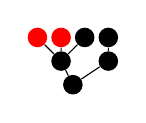
\begin{tikzpicture}[scale=.2]
          \node[circle, scale=0.75, fill] (tid0) at (3,1.5){};
          \node[circle, scale=0.75, fill] (tid1) at (2.25,3){};
          \node[circle, scale=0.75, fill, red] (tid3) at (0.75,4.5){};
          \node[circle, scale=0.75, fill, red] (tid4) at (2.25,4.5){};
          \node[circle, scale=0.75, fill] (tid5) at (3.75,4.5){};
          \draw[](tid1) -- (tid3);
          \draw[](tid1) -- (tid4);
          \draw[](tid1) -- (tid5);
          \node[circle, scale=0.75, fill] (tid2) at (5.25,3){};
          \node[circle, scale=0.75, fill] (tid6) at (5.25,4.5){};
          \draw[](tid2) -- (tid6);
          \draw[](tid0) -- (tid1);
          \draw[](tid0) -- (tid2);
        \end{tikzpicture}
        \nodepart{two}
        \footnotesize{4.75}
        \nodepart{three}
        \footnotesize{$50\:50$}
      };
      & 
      \node[draw=black, rectangle split,  rectangle split parts=3] (sn0x1056fb0){
        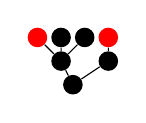
\begin{tikzpicture}[scale=.2]
          \node[circle, scale=0.75, fill] (tid0) at (3,1.5){};
          \node[circle, scale=0.75, fill] (tid1) at (2.25,3){};
          \node[circle, scale=0.75, fill, red] (tid3) at (0.75,4.5){};
          \node[circle, scale=0.75, fill] (tid4) at (2.25,4.5){};
          \node[circle, scale=0.75, fill] (tid5) at (3.75,4.5){};
          \draw[](tid1) -- (tid3);
          \draw[](tid1) -- (tid4);
          \draw[](tid1) -- (tid5);
          \node[circle, scale=0.75, fill] (tid2) at (5.25,3){};
          \node[circle, scale=0.75, fill, red] (tid6) at (5.25,4.5){};
          \draw[](tid2) -- (tid6);
          \draw[](tid0) -- (tid1);
          \draw[](tid0) -- (tid2);
        \end{tikzpicture}
        \nodepart{two}
        \footnotesize{4.75}
        \nodepart{three}
        \footnotesize{$50\:50$}
      };
      & 
      \node[draw=black, rectangle split,  rectangle split parts=3] (sn0x1058f50){
        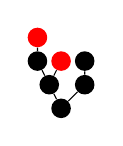
\begin{tikzpicture}[scale=.2]
          \node[circle, scale=0.75, fill] (tid0) at (2.25,1.5){};
          \node[circle, scale=0.75, fill] (tid1) at (1.5,3){};
          \node[circle, scale=0.75, fill] (tid3) at (0.75,4.5){};
          \node[circle, scale=0.75, fill, red] (tid6) at (0.75,6){};
          \draw[](tid3) -- (tid6);
          \node[circle, scale=0.75, fill, red] (tid4) at (2.25,4.5){};
          \draw[](tid1) -- (tid3);
          \draw[](tid1) -- (tid4);
          \node[circle, scale=0.75, fill] (tid2) at (3.75,3){};
          \node[circle, scale=0.75, fill] (tid5) at (3.75,4.5){};
          \draw[](tid2) -- (tid5);
          \draw[](tid0) -- (tid1);
          \draw[](tid0) -- (tid2);
        \end{tikzpicture}
        \nodepart{two}
        \footnotesize{4.84375}
        \nodepart{three}
        \footnotesize{$50\:25\:25$}
      };
      & 
      \node[draw=black, rectangle split,  rectangle split parts=3] (sn0x1058a50){
        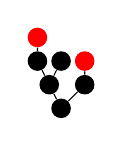
\begin{tikzpicture}[scale=.2]
          \node[circle, scale=0.75, fill] (tid0) at (2.25,1.5){};
          \node[circle, scale=0.75, fill] (tid1) at (1.5,3){};
          \node[circle, scale=0.75, fill] (tid3) at (0.75,4.5){};
          \node[circle, scale=0.75, fill, red] (tid6) at (0.75,6){};
          \draw[](tid3) -- (tid6);
          \node[circle, scale=0.75, fill] (tid4) at (2.25,4.5){};
          \draw[](tid1) -- (tid3);
          \draw[](tid1) -- (tid4);
          \node[circle, scale=0.75, fill] (tid2) at (3.75,3){};
          \node[circle, scale=0.75, fill, red] (tid5) at (3.75,4.5){};
          \draw[](tid2) -- (tid5);
          \draw[](tid0) -- (tid1);
          \draw[](tid0) -- (tid2);
        \end{tikzpicture}
        \nodepart{two}
        \footnotesize{4.84375}
        \nodepart{three}
        \footnotesize{$50\:50$}
      };
      & 
      \node[draw=black, rectangle split,  rectangle split parts=3] (sn0x10597a0){
        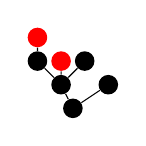
\begin{tikzpicture}[scale=.2]
          \node[circle, scale=0.75, fill] (tid0) at (3,1.5){};
          \node[circle, scale=0.75, fill] (tid1) at (2.25,3){};
          \node[circle, scale=0.75, fill] (tid3) at (0.75,4.5){};
          \node[circle, scale=0.75, fill, red] (tid6) at (0.75,6){};
          \draw[](tid3) -- (tid6);
          \node[circle, scale=0.75, fill, red] (tid4) at (2.25,4.5){};
          \node[circle, scale=0.75, fill] (tid5) at (3.75,4.5){};
          \draw[](tid1) -- (tid3);
          \draw[](tid1) -- (tid4);
          \draw[](tid1) -- (tid5);
          \node[circle, scale=0.75, fill] (tid2) at (5.25,3){};
          \draw[](tid0) -- (tid1);
          \draw[](tid0) -- (tid2);
        \end{tikzpicture}
        \nodepart{two}
        \footnotesize{4.84375}
        \nodepart{three}
        \footnotesize{$50\:50$}
      };
      & 
      \\
    };
  \end{scope}
  \begin{scope}[yshift=\leveltopIIIIII cm]
    \matrix (line6) [column sep=1cm] {
      \node[draw=black, rectangle split,  rectangle split parts=3] (sn0x1053920){
        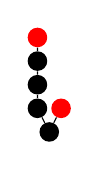
\begin{tikzpicture}[scale=.2]
          \node[circle, scale=0.75, fill] (tid0) at (1.5,1.5){};
          \node[circle, scale=0.75, fill] (tid1) at (0.75,3){};
          \node[circle, scale=0.75, fill] (tid3) at (0.75,4.5){};
          \node[circle, scale=0.75, fill] (tid4) at (0.75,6){};
          \node[circle, scale=0.75, fill, red] (tid5) at (0.75,7.5){};
          \draw[](tid4) -- (tid5);
          \draw[](tid3) -- (tid4);
          \draw[](tid1) -- (tid3);
          \node[circle, scale=0.75, fill, red] (tid2) at (2.25,3){};
          \draw[](tid0) -- (tid1);
          \draw[](tid0) -- (tid2);
        \end{tikzpicture}
        \nodepart{two}
        \footnotesize{5.0625}
        \nodepart{three}
        \footnotesize{$50\:50$}
      };
      & 
      \node[draw=black, rectangle split,  rectangle split parts=3] (sn0x1053bc0){
        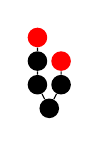
\begin{tikzpicture}[scale=.2]
          \node[circle, scale=0.75, fill] (tid0) at (1.5,1.5){};
          \node[circle, scale=0.75, fill] (tid1) at (0.75,3){};
          \node[circle, scale=0.75, fill] (tid3) at (0.75,4.5){};
          \node[circle, scale=0.75, fill, red] (tid5) at (0.75,6){};
          \draw[](tid3) -- (tid5);
          \draw[](tid1) -- (tid3);
          \node[circle, scale=0.75, fill] (tid2) at (2.25,3){};
          \node[circle, scale=0.75, fill, red] (tid4) at (2.25,4.5){};
          \draw[](tid2) -- (tid4);
          \draw[](tid0) -- (tid1);
          \draw[](tid0) -- (tid2);
        \end{tikzpicture}
        \nodepart{two}
        \footnotesize{4.4375}
        \nodepart{three}
        \footnotesize{$50\:50$}
      };
      & 
      \node[draw=black, rectangle split,  rectangle split parts=3] (sn0x1056090){
        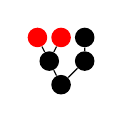
\begin{tikzpicture}[scale=.2]
          \node[circle, scale=0.75, fill] (tid0) at (2.25,1.5){};
          \node[circle, scale=0.75, fill] (tid1) at (1.5,3){};
          \node[circle, scale=0.75, fill, red] (tid3) at (0.75,4.5){};
          \node[circle, scale=0.75, fill, red] (tid4) at (2.25,4.5){};
          \draw[](tid1) -- (tid3);
          \draw[](tid1) -- (tid4);
          \node[circle, scale=0.75, fill] (tid2) at (3.75,3){};
          \node[circle, scale=0.75, fill] (tid5) at (3.75,4.5){};
          \draw[](tid2) -- (tid5);
          \draw[](tid0) -- (tid1);
          \draw[](tid0) -- (tid2);
        \end{tikzpicture}
        \nodepart{two}
        \footnotesize{4.25}
        \nodepart{three}
        \footnotesize{$1$}
      };
      & 
      \node[draw=black, rectangle split,  rectangle split parts=3] (sn0x1056160){
        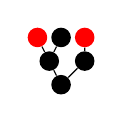
\begin{tikzpicture}[scale=.2]
          \node[circle, scale=0.75, fill] (tid0) at (2.25,1.5){};
          \node[circle, scale=0.75, fill] (tid1) at (1.5,3){};
          \node[circle, scale=0.75, fill, red] (tid3) at (0.75,4.5){};
          \node[circle, scale=0.75, fill] (tid4) at (2.25,4.5){};
          \draw[](tid1) -- (tid3);
          \draw[](tid1) -- (tid4);
          \node[circle, scale=0.75, fill] (tid2) at (3.75,3){};
          \node[circle, scale=0.75, fill, red] (tid5) at (3.75,4.5){};
          \draw[](tid2) -- (tid5);
          \draw[](tid0) -- (tid1);
          \draw[](tid0) -- (tid2);
        \end{tikzpicture}
        \nodepart{two}
        \footnotesize{4.25}
        \nodepart{three}
        \footnotesize{$50\:50$}
      };
      & 
      \node[draw=black, rectangle split,  rectangle split parts=3] (sn0x1057630){
        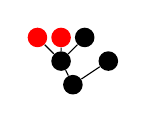
\begin{tikzpicture}[scale=.2]
          \node[circle, scale=0.75, fill] (tid0) at (3,1.5){};
          \node[circle, scale=0.75, fill] (tid1) at (2.25,3){};
          \node[circle, scale=0.75, fill, red] (tid3) at (0.75,4.5){};
          \node[circle, scale=0.75, fill, red] (tid4) at (2.25,4.5){};
          \node[circle, scale=0.75, fill] (tid5) at (3.75,4.5){};
          \draw[](tid1) -- (tid3);
          \draw[](tid1) -- (tid4);
          \draw[](tid1) -- (tid5);
          \node[circle, scale=0.75, fill] (tid2) at (5.25,3){};
          \draw[](tid0) -- (tid1);
          \draw[](tid0) -- (tid2);
        \end{tikzpicture}
        \nodepart{two}
        \footnotesize{4.25}
        \nodepart{three}
        \footnotesize{$1$}
      };
      & 
      \node[draw=black, rectangle split,  rectangle split parts=3] (sn0x1058b20){
        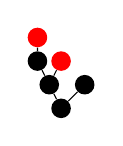
\begin{tikzpicture}[scale=.2]
          \node[circle, scale=0.75, fill] (tid0) at (2.25,1.5){};
          \node[circle, scale=0.75, fill] (tid1) at (1.5,3){};
          \node[circle, scale=0.75, fill] (tid3) at (0.75,4.5){};
          \node[circle, scale=0.75, fill, red] (tid5) at (0.75,6){};
          \draw[](tid3) -- (tid5);
          \node[circle, scale=0.75, fill, red] (tid4) at (2.25,4.5){};
          \draw[](tid1) -- (tid3);
          \draw[](tid1) -- (tid4);
          \node[circle, scale=0.75, fill] (tid2) at (3.75,3){};
          \draw[](tid0) -- (tid1);
          \draw[](tid0) -- (tid2);
        \end{tikzpicture}
        \nodepart{two}
        \footnotesize{4.4375}
        \nodepart{three}
        \footnotesize{$50\:50$}
      };
      & 
      \\
    };
  \end{scope}
  \begin{scope}[yshift=\leveltopIIIIIII cm]
    \matrix (line7) [column sep=1cm] {
      \node[draw=black, rectangle split,  rectangle split parts=3] (sn0x10540d0){
        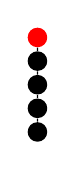
\begin{tikzpicture}[scale=.2]
          \node[circle, scale=0.75, fill] (tid0) at (0.75,1.5){};
          \node[circle, scale=0.75, fill] (tid1) at (0.75,3){};
          \node[circle, scale=0.75, fill] (tid2) at (0.75,4.5){};
          \node[circle, scale=0.75, fill] (tid3) at (0.75,6){};
          \node[circle, scale=0.75, fill, red] (tid4) at (0.75,7.5){};
          \draw[](tid3) -- (tid4);
          \draw[](tid2) -- (tid3);
          \draw[](tid1) -- (tid2);
          \draw[](tid0) -- (tid1);
        \end{tikzpicture}
        \nodepart{two}
        \footnotesize{5}
        \nodepart{three}
        \footnotesize{$1$}
      };
      & 
      \node[draw=black, rectangle split,  rectangle split parts=3] (sn0x1054480){
        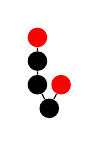
\begin{tikzpicture}[scale=.2]
          \node[circle, scale=0.75, fill] (tid0) at (1.5,1.5){};
          \node[circle, scale=0.75, fill] (tid1) at (0.75,3){};
          \node[circle, scale=0.75, fill] (tid3) at (0.75,4.5){};
          \node[circle, scale=0.75, fill, red] (tid4) at (0.75,6){};
          \draw[](tid3) -- (tid4);
          \draw[](tid1) -- (tid3);
          \node[circle, scale=0.75, fill, red] (tid2) at (2.25,3){};
          \draw[](tid0) -- (tid1);
          \draw[](tid0) -- (tid2);
        \end{tikzpicture}
        \nodepart{two}
        \footnotesize{4.125}
        \nodepart{three}
        \footnotesize{$50\:50$}
      };
      & 
      \node[draw=black, rectangle split,  rectangle split parts=3] (sn0x1055dd0){
        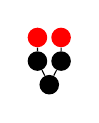
\begin{tikzpicture}[scale=.2]
          \node[circle, scale=0.75, fill] (tid0) at (1.5,1.5){};
          \node[circle, scale=0.75, fill] (tid1) at (0.75,3){};
          \node[circle, scale=0.75, fill, red] (tid3) at (0.75,4.5){};
          \draw[](tid1) -- (tid3);
          \node[circle, scale=0.75, fill] (tid2) at (2.25,3){};
          \node[circle, scale=0.75, fill, red] (tid4) at (2.25,4.5){};
          \draw[](tid2) -- (tid4);
          \draw[](tid0) -- (tid1);
          \draw[](tid0) -- (tid2);
        \end{tikzpicture}
        \nodepart{two}
        \footnotesize{3.75}
        \nodepart{three}
        \footnotesize{$1$}
      };
      & 
      \node[draw=black, rectangle split,  rectangle split parts=3] (sn0x10568c0){
        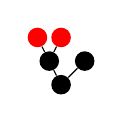
\begin{tikzpicture}[scale=.2]
          \node[circle, scale=0.75, fill] (tid0) at (2.25,1.5){};
          \node[circle, scale=0.75, fill] (tid1) at (1.5,3){};
          \node[circle, scale=0.75, fill, red] (tid3) at (0.75,4.5){};
          \node[circle, scale=0.75, fill, red] (tid4) at (2.25,4.5){};
          \draw[](tid1) -- (tid3);
          \draw[](tid1) -- (tid4);
          \node[circle, scale=0.75, fill] (tid2) at (3.75,3){};
          \draw[](tid0) -- (tid1);
          \draw[](tid0) -- (tid2);
        \end{tikzpicture}
        \nodepart{two}
        \footnotesize{3.75}
        \nodepart{three}
        \footnotesize{$1$}
      };
      & 
      \\
    };
  \end{scope}
  \begin{scope}[yshift=\leveltopIIIIIIII cm]
    \matrix (line8) [column sep=1cm] {
      \node[draw=black, rectangle split,  rectangle split parts=3] (sn0x1054550){
        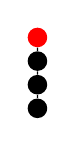
\begin{tikzpicture}[scale=.2]
          \node[circle, scale=0.75, fill] (tid0) at (0.75,1.5){};
          \node[circle, scale=0.75, fill] (tid1) at (0.75,3){};
          \node[circle, scale=0.75, fill] (tid2) at (0.75,4.5){};
          \node[circle, scale=0.75, fill, red] (tid3) at (0.75,6){};
          \draw[](tid2) -- (tid3);
          \draw[](tid1) -- (tid2);
          \draw[](tid0) -- (tid1);
        \end{tikzpicture}
        \nodepart{two}
        \footnotesize{4}
        \nodepart{three}
        \footnotesize{$1$}
      };
      & 
      \node[draw=black, rectangle split,  rectangle split parts=3] (sn0x1055270){
        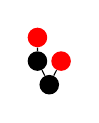
\begin{tikzpicture}[scale=.2]
          \node[circle, scale=0.75, fill] (tid0) at (1.5,1.5){};
          \node[circle, scale=0.75, fill] (tid1) at (0.75,3){};
          \node[circle, scale=0.75, fill, red] (tid3) at (0.75,4.5){};
          \draw[](tid1) -- (tid3);
          \node[circle, scale=0.75, fill, red] (tid2) at (2.25,3){};
          \draw[](tid0) -- (tid1);
          \draw[](tid0) -- (tid2);
        \end{tikzpicture}
        \nodepart{two}
        \footnotesize{3.25}
        \nodepart{three}
        \footnotesize{$50\:50$}
      };
      & 
      \\
    };
  \end{scope}
  \begin{scope}[yshift=\leveltopIIIIIIIII cm]
    \matrix (line9) [column sep=1cm] {
      \node[draw=black, rectangle split,  rectangle split parts=3] (sn0x1054a50){
        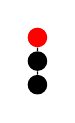
\begin{tikzpicture}[scale=.2]
          \node[circle, scale=0.75, fill] (tid0) at (0.75,1.5){};
          \node[circle, scale=0.75, fill] (tid1) at (0.75,3){};
          \node[circle, scale=0.75, fill, red] (tid2) at (0.75,4.5){};
          \draw[](tid1) -- (tid2);
          \draw[](tid0) -- (tid1);
        \end{tikzpicture}
        \nodepart{two}
        \footnotesize{3}
        \nodepart{three}
        \footnotesize{$1$}
      };
      & 
      \node[draw=black, rectangle split,  rectangle split parts=3] (sn0x1054cb0){
        
\begin{tikzpicture}[scale=.2]
          \node[circle, scale=0.75, fill] (tid0) at (1.5,1.5){};
          \node[circle, scale=0.75, fill, red] (tid1) at (0.75,3){};
          \node[circle, scale=0.75, fill, red] (tid2) at (2.25,3){};
          \draw[](tid0) -- (tid1);
          \draw[](tid0) -- (tid2);
        \end{tikzpicture}
        \nodepart{two}
        \footnotesize{2.5}
        \nodepart{three}
        \footnotesize{$1$}
      };
      & 
      \\
    };
  \end{scope}
  \begin{scope}[yshift=\leveltopIIIIIIIIII cm]
    \matrix (line10) [column sep=1cm] {
      \node[draw=black, rectangle split,  rectangle split parts=3] (sn0x1054b20){
        
\begin{tikzpicture}[scale=.2]
          \node[circle, scale=0.75, fill] (tid0) at (0.75,1.5){};
          \node[circle, scale=0.75, fill, red] (tid1) at (0.75,3){};
          \draw[](tid0) -- (tid1);
        \end{tikzpicture}
        \nodepart{two}
        \footnotesize{2}
        \nodepart{three}
        \footnotesize{$1$}
      };
      & 
      \\
    };
  \end{scope}
  \begin{scope}[yshift=\leveltopIIIIIIIIIII cm]
    \matrix (line11) [column sep=1cm] {
      \node[draw=black, rectangle split,  rectangle split parts=3] (sn0x10547e0){
        
\begin{tikzpicture}[scale=.2]
          \node[circle, scale=0.75, fill, red] (tid0) at (0.75,1.5){};
        \end{tikzpicture}
        \nodepart{two}
        \footnotesize{1}
        \nodepart{three}
        \footnotesize{$$}
      };
      & 
      \\
    };
  \end{scope}
  \begin{scope}[yshift=\leveltopIIIIIIIIIIII cm]
    \matrix (line12) [column sep=1cm] {
      \\
    };
  \end{scope}
  \draw (sn0x104f980.south) -- (sn0x1050190.north);
  \draw (sn0x104f980.south) -- (sn0x104cb60.north);
  \draw (sn0x104f980.south) -- (sn0x104dd20.north);
  \draw (sn0x1050190.south) -- (sn0x10519d0.north);
  \draw (sn0x1050190.south) -- (sn0x104fbd0.north);
  \draw (sn0x104cb60.south) -- (sn0x105a080.north);
  \draw (sn0x104cb60.south) -- (sn0x104fbd0.north);
  \draw (sn0x104dd20.south) -- (sn0x104fbd0.north);
  \draw (sn0x10519d0.south) -- (sn0x1052250.north);
  \draw (sn0x10519d0.south) -- (sn0x1052960.north);
  \draw (sn0x104fbd0.south) -- (sn0x1052960.north);
  \draw (sn0x104fbd0.south) -- (sn0x10581e0.north);
  \draw (sn0x104fbd0.south) -- (sn0x1058550.north);
  \draw (sn0x105a080.south) -- (sn0x1052960.north);
  \draw (sn0x1052250.south) -- (sn0x10525f0.north);
  \draw (sn0x1052250.south) -- (sn0x1053850.north);
  \draw (sn0x1052960.south) -- (sn0x1053850.north);
  \draw (sn0x1052960.south) -- (sn0x1056b00.north);
  \draw (sn0x1052960.south) -- (sn0x1056fb0.north);
  \draw (sn0x10581e0.south) -- (sn0x1058f50.north);
  \draw (sn0x10581e0.south) -- (sn0x1058a50.north);
  \draw (sn0x10581e0.south) -- (sn0x1056b00.north);
  \draw (sn0x10581e0.south) -- (sn0x1056fb0.north);
  \draw (sn0x1058550.south) -- (sn0x10597a0.north);
  \draw (sn0x1058550.south) -- (sn0x1056fb0.north);
  \draw (sn0x10525f0.south) -- (sn0x1053920.north);
  \draw (sn0x10525f0.south) -- (sn0x1053bc0.north);
  \draw (sn0x1053850.south) -- (sn0x1053bc0.north);
  \draw (sn0x1053850.south) -- (sn0x1056090.north);
  \draw (sn0x1053850.south) -- (sn0x1056160.north);
  \draw (sn0x1056b00.south) -- (sn0x1056090.north);
  \draw (sn0x1056b00.south) -- (sn0x1056160.north);
  \draw (sn0x1056fb0.south) -- (sn0x1056160.north);
  \draw (sn0x1056fb0.south) -- (sn0x1057630.north);
  \draw (sn0x1058f50.south) -- (sn0x1053bc0.north);
  \draw (sn0x1058f50.south) -- (sn0x1056090.north);
  \draw (sn0x1058f50.south) -- (sn0x1056160.north);
  \draw (sn0x1058a50.south) -- (sn0x1058b20.north);
  \draw (sn0x1058a50.south) -- (sn0x1056160.north);
  \draw (sn0x10597a0.south) -- (sn0x1058b20.north);
  \draw (sn0x10597a0.south) -- (sn0x1057630.north);
  \draw (sn0x1053920.south) -- (sn0x10540d0.north);
  \draw (sn0x1053920.south) -- (sn0x1054480.north);
  \draw (sn0x1053bc0.south) -- (sn0x1054480.north);
  \draw (sn0x1053bc0.south) -- (sn0x1055dd0.north);
  \draw (sn0x1056090.south) -- (sn0x1055dd0.north);
  \draw (sn0x1056160.south) -- (sn0x1055dd0.north);
  \draw (sn0x1056160.south) -- (sn0x10568c0.north);
  \draw (sn0x1057630.south) -- (sn0x10568c0.north);
  \draw (sn0x1058b20.south) -- (sn0x1054480.north);
  \draw (sn0x1058b20.south) -- (sn0x10568c0.north);
  \draw (sn0x10540d0.south) -- (sn0x1054550.north);
  \draw (sn0x1054480.south) -- (sn0x1054550.north);
  \draw (sn0x1054480.south) -- (sn0x1055270.north);
  \draw (sn0x1055dd0.south) -- (sn0x1055270.north);
  \draw (sn0x10568c0.south) -- (sn0x1055270.north);
  \draw (sn0x1054550.south) -- (sn0x1054a50.north);
  \draw (sn0x1055270.south) -- (sn0x1054a50.north);
  \draw (sn0x1055270.south) -- (sn0x1054cb0.north);
  \draw (sn0x1054a50.south) -- (sn0x1054b20.north);
  \draw (sn0x1054cb0.south) -- (sn0x1054b20.north);
  \draw (sn0x1054b20.south) -- (sn0x10547e0.north);

  \newcommand{\nd}[4]{
    \node[draw=black, rectangle split, rectangle split parts=3] (n#1#2) {
      $#1/#2$
      \nodepart{two}
      #3
      \nodepart{three}
      #4
    };
  }

  \begin{scope}[yshift=\leveltopI, xshift=70cm, rectangle, draw=black,anchor=south]
    \matrix (test) [column sep=1cm] {
      \nd{5}{6}{6.82812}{50 50};
      \\
    };
  \end{scope}

  \begin{scope}[yshift=\leveltopII, xshift=70cm, rectangle, draw=black,anchor=south]
    \matrix (test) [column sep=1cm] {
      \nd{5}{5}{6.35938}{50 50};
      &
      \nd{4}{6}{6.29688}{1};
      \\
      };
    \end{scope}

    \begin{scope}[yshift=\leveltopIII, xshift=70cm, rectangle, draw=black,anchor=south]
      \matrix (test) [column sep=1cm] {
        \nd{5}{4}{5.92188}{50 50};
        &
        \nd{4}{5}{5.79688}{1};
        \\
      };
    \end{scope}

    \begin{scope}[yshift=\leveltopIIII, xshift=70cm, rectangle, draw=black,anchor=south]
      \matrix (test) [column sep=1cm] {
        \nd{5}{3}{5.54688}{50 50};
        &
        \nd{4}{4}{5.29688}{50 50};
        \\
      };
    \end{scope}

    \begin{scope}[yshift=\leveltopIIIII, xshift=70cm, rectangle, draw=black,anchor=south]
      \matrix (test) [column sep=1cm] {
        \nd{5}{2}{5.25}{50 50};
        &
        \nd{4}{3}{4.84375}{50 50};
        &
        \nd{3}{4}{5.29688}{1};
        \\
      };
    \end{scope}

    \begin{scope}[yshift=\leveltopIIIIII, xshift=70cm, rectangle, draw=black,anchor=south]
      \matrix (test) [column sep=1cm] {
        \nd{5}{1}{5.0625}{50 50};
        &
        \nd{4}{2}{4.4375}{50 50};
        &
        \nd{3}{3}{5.75}{1};
        \\
      };
    \end{scope}

    \begin{scope}[yshift=\leveltopIIIIIII, xshift=70cm, rectangle, draw=black,anchor=south]
      \matrix (test) [column sep=1cm] {
        \nd{5}{0}{5}{50 50};
        &
        \nd{4}{1}{4.125}{50 50};
        &
        \nd{3}{2}{5.25}{1};
        \\
      };
    \end{scope}
    
    \begin{scope}[yshift=\leveltopIIIIIIII, xshift=70cm, rectangle, draw=black,anchor=south]
      \matrix (test) [column sep=1cm] {
        \nd{4}{0}{4}{1};
        &
        \nd{3}{1}{3.25}{50 50};
        \\
      };
    \end{scope}

    \begin{scope}[yshift=\leveltopIIIIIIIII, xshift=70cm, rectangle, draw=black,anchor=south]
      \matrix (test) [column sep=1cm] {
        \nd{3}{0}{3}{1};
        &
        \nd{2}{1}{2.5}{1};
        \\
      };
    \end{scope}

    \begin{scope}[yshift=\leveltopIIIIIIIIII, xshift=70cm, rectangle, draw=black,anchor=south]
      \matrix (test) [column sep=1cm] {
        \nd{2}{0}{2}{1};
        \\
      };
    \end{scope}
    
    \begin{scope}[yshift=\leveltopIIIIIIIIIII, xshift=70cm, rectangle, draw=black,anchor=south]
      \matrix (test) [column sep=1cm] {
        \nd{1}{0}{1}{1};
        \\
      };
    \end{scope}

    \draw (n56.south) -- (n55.north);
    \draw (n56.south) -- (n46.north);
    \draw (n55.south) -- (n54.north);
    \draw (n55.south) -- (n45.north);
    \draw (n46.south) -- (n45.north);
    \draw (n54.south) -- (n53.north);
    \draw (n54.south) -- (n44.north);
    \draw (n45.south) -- (n44.north);
    \draw (n53.south) -- (n52.north);
    \draw (n53.south) -- (n43.north);
    \draw (n44.south) -- (n43.north);
    \draw (n44.south) -- (n34.north);
    \draw (n52.south) -- (n51.north);
    \draw (n52.south) -- (n42.north);
    \draw (n43.south) -- (n42.north);
    \draw (n43.south) -- (n33.north);
    \draw (n34.south) -- (n33.north);
    \draw (n51.south) -- (n50.north);
    \draw (n51.south) -- (n41.north);
    \draw (n42.south) -- (n41.north);
    \draw (n42.south) -- (n32.north);
    \draw (n33.south) -- (n32.north);
    \draw (n32.south) -- (n31.north);
    \draw (n50.south) -- (n40.north);
    \draw (n41.south) -- (n40.north);
    \draw (n41.south) -- (n31.north);
    \draw (n40.south) -- (n30.north);
    \draw (n31.south) -- (n30.north);
    \draw (n31.south) -- (n21.north);
    \draw (n30.south) -- (n20.north);
    \draw (n21.south) -- (n20.north);
    \draw (n20.south) -- (n10.north);

\end{tikzpicture}

%%% Local Variables:
%%% TeX-master: "thesis/thesis.tex"
%%% End: 
\renewcommand{\leveltopI}{-15cm + \leveltop}
\renewcommand{\leveltopII}{-15cm + \leveltopI}
\renewcommand{\leveltopIII}{-15cm + \leveltopII}
\renewcommand{\leveltopIIII}{-15cm + \leveltopIII}
\renewcommand{\leveltopIIIII}{-15cm + \leveltopIIII}
\renewcommand{\leveltopIIIIII}{-15cm + \leveltopIIIII}
\renewcommand{\leveltopIIIIIII}{-15cm + \leveltopIIIIII}
\renewcommand{\leveltopIIIIIIII}{-15cm + \leveltopIIIIIII}
\renewcommand{\leveltopIIIIIIIII}{-15cm + \leveltopIIIIIIII}
\renewcommand{\leveltopIIIIIIIIII}{-15cm + \leveltopIIIIIIIII}
\renewcommand{\leveltopIIIIIIIIIII}{-15cm + \leveltopIIIIIIIIII}
% \begin{tikzpicture}[scale=.2, anchor=south]
%   \begin{scope}[yshift=\leveltopI cm]
%     \matrix (line1) [column sep=1cm] {
%       \node[draw=black, rectangle split,  rectangle split parts=3] (sn0x1050af0){
%         \begin{tikzpicture}[scale=.2]
%           \node[circle, scale=0.75, fill] (tid0) at (3.75,1.5){};
%           \node[circle, scale=0.75, fill] (tid1) at (2.25,3){};
%           \node[circle, scale=0.75, fill] (tid3) at (0.75,4.5){};
%           \node[circle, scale=0.75, fill, red] (tid7) at (0.75,6){};
%           \draw[](tid3) -- (tid7);
%           \node[circle, scale=0.75, fill] (tid4) at (2.25,4.5){};
%           \node[circle, scale=0.75, fill] (tid5) at (3.75,4.5){};
%           \draw[](tid1) -- (tid3);
%           \draw[](tid1) -- (tid4);
%           \draw[](tid1) -- (tid5);
%           \node[circle, scale=0.75, fill] (tid2) at (6,3){};
%           \node[circle, scale=0.75, fill] (tid6) at (6,4.5){};
%           \node[circle, scale=0.75, fill] (tid8) at (5.25,6){};
%           \node[circle, scale=0.75, fill, red] (tid10) at (5.25,7.5){};
%           \draw[](tid8) -- (tid10);
%           \node[circle, scale=0.75, fill] (tid9) at (6.75,6){};
%           \draw[](tid6) -- (tid8);
%           \draw[](tid6) -- (tid9);
%           \draw[](tid2) -- (tid6);
%           \draw[](tid0) -- (tid1);
%           \draw[](tid0) -- (tid2);
%         \end{tikzpicture}
%         \nodepart{two}
%         \footnotesize{6.82812}
%         \nodepart{three}
%         \footnotesize{$50\:50$}
%       };
%       & 
%       \\
%     };
%   \end{scope}
%   \begin{scope}[yshift=\leveltopII cm]
%     \matrix (line2) [column sep=1cm] {
%       \node[draw=black, rectangle split,  rectangle split parts=3] (sn0x105a150){
%         \begin{tikzpicture}[scale=.2]
%           \node[circle, scale=0.75, fill] (tid0) at (3.75,1.5){};
%           \node[circle, scale=0.75, fill] (tid1) at (1.5,3){};
%           \node[circle, scale=0.75, fill] (tid3) at (1.5,4.5){};
%           \node[circle, scale=0.75, fill] (tid7) at (0.75,6){};
%           \node[circle, scale=0.75, fill, red] (tid9) at (0.75,7.5){};
%           \draw[](tid7) -- (tid9);
%           \node[circle, scale=0.75, fill, red] (tid8) at (2.25,6){};
%           \draw[](tid3) -- (tid7);
%           \draw[](tid3) -- (tid8);
%           \draw[](tid1) -- (tid3);
%           \node[circle, scale=0.75, fill] (tid2) at (5.25,3){};
%           \node[circle, scale=0.75, fill] (tid4) at (3.75,4.5){};
%           \node[circle, scale=0.75, fill] (tid5) at (5.25,4.5){};
%           \node[circle, scale=0.75, fill] (tid6) at (6.75,4.5){};
%           \draw[](tid2) -- (tid4);
%           \draw[](tid2) -- (tid5);
%           \draw[](tid2) -- (tid6);
%           \draw[](tid0) -- (tid1);
%           \draw[](tid0) -- (tid2);
%         \end{tikzpicture}
%         \nodepart{two}
%         \footnotesize{6.35938}
%         \nodepart{three}
%         \footnotesize{$50\:50$}
%       };
%       & 
%       \node[draw=black, rectangle split,  rectangle split parts=3] (sn0x104cb60){
%         \begin{tikzpicture}[scale=.2]
%           \node[circle, scale=0.75, fill] (tid0) at (3.75,1.5){};
%           \node[circle, scale=0.75, fill] (tid1) at (2.25,3){};
%           \node[circle, scale=0.75, fill] (tid3) at (0.75,4.5){};
%           \node[circle, scale=0.75, fill, red] (tid7) at (0.75,6){};
%           \draw[](tid3) -- (tid7);
%           \node[circle, scale=0.75, fill] (tid4) at (2.25,4.5){};
%           \node[circle, scale=0.75, fill] (tid5) at (3.75,4.5){};
%           \draw[](tid1) -- (tid3);
%           \draw[](tid1) -- (tid4);
%           \draw[](tid1) -- (tid5);
%           \node[circle, scale=0.75, fill] (tid2) at (6,3){};
%           \node[circle, scale=0.75, fill] (tid6) at (6,4.5){};
%           \node[circle, scale=0.75, fill, red] (tid8) at (5.25,6){};
%           \node[circle, scale=0.75, fill] (tid9) at (6.75,6){};
%           \draw[](tid6) -- (tid8);
%           \draw[](tid6) -- (tid9);
%           \draw[](tid2) -- (tid6);
%           \draw[](tid0) -- (tid1);
%           \draw[](tid0) -- (tid2);
%         \end{tikzpicture}
%         \nodepart{two}
%         \footnotesize{6.29688}
%         \nodepart{three}
%         \footnotesize{$50\:50$}
%       };
%       & 
%       \\
%     };
%   \end{scope}
%   \begin{scope}[yshift=\leveltopIII cm]
%     \matrix (line3) [column sep=1cm] {
%       \node[draw=black, rectangle split,  rectangle split parts=3] (sn0x10519d0){
%         \begin{tikzpicture}[scale=.2]
%           \node[circle, scale=0.75, fill] (tid0) at (3,1.5){};
%           \node[circle, scale=0.75, fill] (tid1) at (2.25,3){};
%           \node[circle, scale=0.75, fill, red] (tid3) at (0.75,4.5){};
%           \node[circle, scale=0.75, fill] (tid4) at (2.25,4.5){};
%           \node[circle, scale=0.75, fill] (tid5) at (3.75,4.5){};
%           \draw[](tid1) -- (tid3);
%           \draw[](tid1) -- (tid4);
%           \draw[](tid1) -- (tid5);
%           \node[circle, scale=0.75, fill] (tid2) at (5.25,3){};
%           \node[circle, scale=0.75, fill] (tid6) at (5.25,4.5){};
%           \node[circle, scale=0.75, fill] (tid7) at (5.25,6){};
%           \node[circle, scale=0.75, fill, red] (tid8) at (5.25,7.5){};
%           \draw[](tid7) -- (tid8);
%           \draw[](tid6) -- (tid7);
%           \draw[](tid2) -- (tid6);
%           \draw[](tid0) -- (tid1);
%           \draw[](tid0) -- (tid2);
%         \end{tikzpicture}
%         \nodepart{two}
%         \footnotesize{5.92188}
%         \nodepart{three}
%         \footnotesize{$50\:50$}
%       };
%       & 
%       \node[draw=black, rectangle split,  rectangle split parts=3] (sn0x105a080){
%         \begin{tikzpicture}[scale=.2]
%           \node[circle, scale=0.75, fill] (tid0) at (3.75,1.5){};
%           \node[circle, scale=0.75, fill] (tid1) at (2.25,3){};
%           \node[circle, scale=0.75, fill] (tid3) at (0.75,4.5){};
%           \node[circle, scale=0.75, fill] (tid4) at (2.25,4.5){};
%           \node[circle, scale=0.75, fill] (tid5) at (3.75,4.5){};
%           \draw[](tid1) -- (tid3);
%           \draw[](tid1) -- (tid4);
%           \draw[](tid1) -- (tid5);
%           \node[circle, scale=0.75, fill] (tid2) at (6,3){};
%           \node[circle, scale=0.75, fill] (tid6) at (6,4.5){};
%           \node[circle, scale=0.75, fill, red] (tid7) at (5.25,6){};
%           \node[circle, scale=0.75, fill, red] (tid8) at (6.75,6){};
%           \draw[](tid6) -- (tid7);
%           \draw[](tid6) -- (tid8);
%           \draw[](tid2) -- (tid6);
%           \draw[](tid0) -- (tid1);
%           \draw[](tid0) -- (tid2);
%         \end{tikzpicture}
%         \nodepart{two}
%         \footnotesize{5.79688}
%         \nodepart{three}
%         \footnotesize{$1$}
%       };
%       & 
%       \node[draw=black, rectangle split,  rectangle split parts=3] (sn0x104fbd0){
%         \begin{tikzpicture}[scale=.2]
%           \node[circle, scale=0.75, fill] (tid0) at (3,1.5){};
%           \node[circle, scale=0.75, fill] (tid1) at (2.25,3){};
%           \node[circle, scale=0.75, fill] (tid3) at (0.75,4.5){};
%           \node[circle, scale=0.75, fill, red] (tid7) at (0.75,6){};
%           \draw[](tid3) -- (tid7);
%           \node[circle, scale=0.75, fill] (tid4) at (2.25,4.5){};
%           \node[circle, scale=0.75, fill] (tid5) at (3.75,4.5){};
%           \draw[](tid1) -- (tid3);
%           \draw[](tid1) -- (tid4);
%           \draw[](tid1) -- (tid5);
%           \node[circle, scale=0.75, fill] (tid2) at (5.25,3){};
%           \node[circle, scale=0.75, fill] (tid6) at (5.25,4.5){};
%           \node[circle, scale=0.75, fill, red] (tid8) at (5.25,6){};
%           \draw[](tid6) -- (tid8);
%           \draw[](tid2) -- (tid6);
%           \draw[](tid0) -- (tid1);
%           \draw[](tid0) -- (tid2);
%         \end{tikzpicture}
%         \nodepart{two}
%         \footnotesize{5.79688}
%         \nodepart{three}
%         \footnotesize{$50\:33\:17$}
%       };
%       & 
%       \\
%     };
%   \end{scope}
%   \begin{scope}[yshift=\leveltopIIII cm]
%     \matrix (line4) [column sep=1cm] {
%       \node[draw=black, rectangle split,  rectangle split parts=3] (sn0x1052250){
%         \begin{tikzpicture}[scale=.2]
%           \node[circle, scale=0.75, fill] (tid0) at (2.25,1.5){};
%           \node[circle, scale=0.75, fill] (tid1) at (0.75,3){};
%           \node[circle, scale=0.75, fill] (tid3) at (0.75,4.5){};
%           \node[circle, scale=0.75, fill] (tid6) at (0.75,6){};
%           \node[circle, scale=0.75, fill, red] (tid7) at (0.75,7.5){};
%           \draw[](tid6) -- (tid7);
%           \draw[](tid3) -- (tid6);
%           \draw[](tid1) -- (tid3);
%           \node[circle, scale=0.75, fill] (tid2) at (3,3){};
%           \node[circle, scale=0.75, fill, red] (tid4) at (2.25,4.5){};
%           \node[circle, scale=0.75, fill] (tid5) at (3.75,4.5){};
%           \draw[](tid2) -- (tid4);
%           \draw[](tid2) -- (tid5);
%           \draw[](tid0) -- (tid1);
%           \draw[](tid0) -- (tid2);
%         \end{tikzpicture}
%         \nodepart{two}
%         \footnotesize{5.54688}
%         \nodepart{three}
%         \footnotesize{$50\:50$}
%       };
%       & 
%       \node[draw=black, rectangle split,  rectangle split parts=3] (sn0x1052960){
%         \begin{tikzpicture}[scale=.2]
%           \node[circle, scale=0.75, fill] (tid0) at (3,1.5){};
%           \node[circle, scale=0.75, fill] (tid1) at (2.25,3){};
%           \node[circle, scale=0.75, fill, red] (tid3) at (0.75,4.5){};
%           \node[circle, scale=0.75, fill] (tid4) at (2.25,4.5){};
%           \node[circle, scale=0.75, fill] (tid5) at (3.75,4.5){};
%           \draw[](tid1) -- (tid3);
%           \draw[](tid1) -- (tid4);
%           \draw[](tid1) -- (tid5);
%           \node[circle, scale=0.75, fill] (tid2) at (5.25,3){};
%           \node[circle, scale=0.75, fill] (tid6) at (5.25,4.5){};
%           \node[circle, scale=0.75, fill, red] (tid7) at (5.25,6){};
%           \draw[](tid6) -- (tid7);
%           \draw[](tid2) -- (tid6);
%           \draw[](tid0) -- (tid1);
%           \draw[](tid0) -- (tid2);
%         \end{tikzpicture}
%         \nodepart{two}
%         \footnotesize{5.29688}
%         \nodepart{three}
%         \footnotesize{$50\:33\:17$}
%       };
%       & 
%       \node[draw=black, rectangle split,  rectangle split parts=3] (sn0x10581e0){
%         \begin{tikzpicture}[scale=.2]
%           \node[circle, scale=0.75, fill] (tid0) at (3,1.5){};
%           \node[circle, scale=0.75, fill] (tid1) at (2.25,3){};
%           \node[circle, scale=0.75, fill] (tid3) at (0.75,4.5){};
%           \node[circle, scale=0.75, fill, red] (tid7) at (0.75,6){};
%           \draw[](tid3) -- (tid7);
%           \node[circle, scale=0.75, fill, red] (tid4) at (2.25,4.5){};
%           \node[circle, scale=0.75, fill] (tid5) at (3.75,4.5){};
%           \draw[](tid1) -- (tid3);
%           \draw[](tid1) -- (tid4);
%           \draw[](tid1) -- (tid5);
%           \node[circle, scale=0.75, fill] (tid2) at (5.25,3){};
%           \node[circle, scale=0.75, fill] (tid6) at (5.25,4.5){};
%           \draw[](tid2) -- (tid6);
%           \draw[](tid0) -- (tid1);
%           \draw[](tid0) -- (tid2);
%         \end{tikzpicture}
%         \nodepart{two}
%         \footnotesize{5.29688}
%         \nodepart{three}
%         \footnotesize{$33\:17\:25\:25$}
%       };
%       & 
%       \node[draw=black, rectangle split,  rectangle split parts=3] (sn0x1058550){
%         \begin{tikzpicture}[scale=.2]
%           \node[circle, scale=0.75, fill] (tid0) at (3,1.5){};
%           \node[circle, scale=0.75, fill] (tid1) at (2.25,3){};
%           \node[circle, scale=0.75, fill] (tid3) at (0.75,4.5){};
%           \node[circle, scale=0.75, fill, red] (tid7) at (0.75,6){};
%           \draw[](tid3) -- (tid7);
%           \node[circle, scale=0.75, fill] (tid4) at (2.25,4.5){};
%           \node[circle, scale=0.75, fill] (tid5) at (3.75,4.5){};
%           \draw[](tid1) -- (tid3);
%           \draw[](tid1) -- (tid4);
%           \draw[](tid1) -- (tid5);
%           \node[circle, scale=0.75, fill] (tid2) at (5.25,3){};
%           \node[circle, scale=0.75, fill, red] (tid6) at (5.25,4.5){};
%           \draw[](tid2) -- (tid6);
%           \draw[](tid0) -- (tid1);
%           \draw[](tid0) -- (tid2);
%         \end{tikzpicture}
%         \nodepart{two}
%         \footnotesize{5.29688}
%         \nodepart{three}
%         \footnotesize{$50\:50$}
%       };
%       & 
%       \\
%     };
%   \end{scope}
%   \begin{scope}[yshift=\leveltopIIIII cm]
%     \matrix (line5) [column sep=1cm] {
%       \node[draw=black, rectangle split,  rectangle split parts=3] (sn0x10525f0){
%         \begin{tikzpicture}[scale=.2]
%           \node[circle, scale=0.75, fill] (tid0) at (1.5,1.5){};
%           \node[circle, scale=0.75, fill] (tid1) at (0.75,3){};
%           \node[circle, scale=0.75, fill] (tid3) at (0.75,4.5){};
%           \node[circle, scale=0.75, fill] (tid5) at (0.75,6){};
%           \node[circle, scale=0.75, fill, red] (tid6) at (0.75,7.5){};
%           \draw[](tid5) -- (tid6);
%           \draw[](tid3) -- (tid5);
%           \draw[](tid1) -- (tid3);
%           \node[circle, scale=0.75, fill] (tid2) at (2.25,3){};
%           \node[circle, scale=0.75, fill, red] (tid4) at (2.25,4.5){};
%           \draw[](tid2) -- (tid4);
%           \draw[](tid0) -- (tid1);
%           \draw[](tid0) -- (tid2);
%         \end{tikzpicture}
%         \nodepart{two}
%         \footnotesize{5.25}
%         \nodepart{three}
%         \footnotesize{$50\:50$}
%       };
%       & 
%       \node[draw=black, rectangle split,  rectangle split parts=3] (sn0x1053850){
%         \begin{tikzpicture}[scale=.2]
%           \node[circle, scale=0.75, fill] (tid0) at (2.25,1.5){};
%           \node[circle, scale=0.75, fill] (tid1) at (1.5,3){};
%           \node[circle, scale=0.75, fill, red] (tid3) at (0.75,4.5){};
%           \node[circle, scale=0.75, fill] (tid4) at (2.25,4.5){};
%           \draw[](tid1) -- (tid3);
%           \draw[](tid1) -- (tid4);
%           \node[circle, scale=0.75, fill] (tid2) at (3.75,3){};
%           \node[circle, scale=0.75, fill] (tid5) at (3.75,4.5){};
%           \node[circle, scale=0.75, fill, red] (tid6) at (3.75,6){};
%           \draw[](tid5) -- (tid6);
%           \draw[](tid2) -- (tid5);
%           \draw[](tid0) -- (tid1);
%           \draw[](tid0) -- (tid2);
%         \end{tikzpicture}
%         \nodepart{two}
%         \footnotesize{4.84375}
%         \nodepart{three}
%         \footnotesize{$50\:25\:25$}
%       };
%       & 
%       \node[draw=black, rectangle split,  rectangle split parts=3] (sn0x1056b00){
%         \begin{tikzpicture}[scale=.2]
%           \node[circle, scale=0.75, fill] (tid0) at (3,1.5){};
%           \node[circle, scale=0.75, fill] (tid1) at (2.25,3){};
%           \node[circle, scale=0.75, fill, red] (tid3) at (0.75,4.5){};
%           \node[circle, scale=0.75, fill, red] (tid4) at (2.25,4.5){};
%           \node[circle, scale=0.75, fill] (tid5) at (3.75,4.5){};
%           \draw[](tid1) -- (tid3);
%           \draw[](tid1) -- (tid4);
%           \draw[](tid1) -- (tid5);
%           \node[circle, scale=0.75, fill] (tid2) at (5.25,3){};
%           \node[circle, scale=0.75, fill] (tid6) at (5.25,4.5){};
%           \draw[](tid2) -- (tid6);
%           \draw[](tid0) -- (tid1);
%           \draw[](tid0) -- (tid2);
%         \end{tikzpicture}
%         \nodepart{two}
%         \footnotesize{4.75}
%         \nodepart{three}
%         \footnotesize{$50\:50$}
%       };
%       & 
%       \node[draw=black, rectangle split,  rectangle split parts=3] (sn0x1056fb0){
%         \begin{tikzpicture}[scale=.2]
%           \node[circle, scale=0.75, fill] (tid0) at (3,1.5){};
%           \node[circle, scale=0.75, fill] (tid1) at (2.25,3){};
%           \node[circle, scale=0.75, fill, red] (tid3) at (0.75,4.5){};
%           \node[circle, scale=0.75, fill] (tid4) at (2.25,4.5){};
%           \node[circle, scale=0.75, fill] (tid5) at (3.75,4.5){};
%           \draw[](tid1) -- (tid3);
%           \draw[](tid1) -- (tid4);
%           \draw[](tid1) -- (tid5);
%           \node[circle, scale=0.75, fill] (tid2) at (5.25,3){};
%           \node[circle, scale=0.75, fill, red] (tid6) at (5.25,4.5){};
%           \draw[](tid2) -- (tid6);
%           \draw[](tid0) -- (tid1);
%           \draw[](tid0) -- (tid2);
%         \end{tikzpicture}
%         \nodepart{two}
%         \footnotesize{4.75}
%         \nodepart{three}
%         \footnotesize{$50\:50$}
%       };
%       & 
%       \node[draw=black, rectangle split,  rectangle split parts=3] (sn0x1058f50){
%         \begin{tikzpicture}[scale=.2]
%           \node[circle, scale=0.75, fill] (tid0) at (2.25,1.5){};
%           \node[circle, scale=0.75, fill] (tid1) at (1.5,3){};
%           \node[circle, scale=0.75, fill] (tid3) at (0.75,4.5){};
%           \node[circle, scale=0.75, fill, red] (tid6) at (0.75,6){};
%           \draw[](tid3) -- (tid6);
%           \node[circle, scale=0.75, fill, red] (tid4) at (2.25,4.5){};
%           \draw[](tid1) -- (tid3);
%           \draw[](tid1) -- (tid4);
%           \node[circle, scale=0.75, fill] (tid2) at (3.75,3){};
%           \node[circle, scale=0.75, fill] (tid5) at (3.75,4.5){};
%           \draw[](tid2) -- (tid5);
%           \draw[](tid0) -- (tid1);
%           \draw[](tid0) -- (tid2);
%         \end{tikzpicture}
%         \nodepart{two}
%         \footnotesize{4.84375}
%         \nodepart{three}
%         \footnotesize{$50\:25\:25$}
%       };
%       & 
%       \node[draw=black, rectangle split,  rectangle split parts=3] (sn0x1058a50){
%         \begin{tikzpicture}[scale=.2]
%           \node[circle, scale=0.75, fill] (tid0) at (2.25,1.5){};
%           \node[circle, scale=0.75, fill] (tid1) at (1.5,3){};
%           \node[circle, scale=0.75, fill] (tid3) at (0.75,4.5){};
%           \node[circle, scale=0.75, fill, red] (tid6) at (0.75,6){};
%           \draw[](tid3) -- (tid6);
%           \node[circle, scale=0.75, fill] (tid4) at (2.25,4.5){};
%           \draw[](tid1) -- (tid3);
%           \draw[](tid1) -- (tid4);
%           \node[circle, scale=0.75, fill] (tid2) at (3.75,3){};
%           \node[circle, scale=0.75, fill, red] (tid5) at (3.75,4.5){};
%           \draw[](tid2) -- (tid5);
%           \draw[](tid0) -- (tid1);
%           \draw[](tid0) -- (tid2);
%         \end{tikzpicture}
%         \nodepart{two}
%         \footnotesize{4.84375}
%         \nodepart{three}
%         \footnotesize{$50\:50$}
%       };
%       & 
%       \node[draw=black, rectangle split,  rectangle split parts=3] (sn0x10597a0){
%         \begin{tikzpicture}[scale=.2]
%           \node[circle, scale=0.75, fill] (tid0) at (3,1.5){};
%           \node[circle, scale=0.75, fill] (tid1) at (2.25,3){};
%           \node[circle, scale=0.75, fill] (tid3) at (0.75,4.5){};
%           \node[circle, scale=0.75, fill, red] (tid6) at (0.75,6){};
%           \draw[](tid3) -- (tid6);
%           \node[circle, scale=0.75, fill, red] (tid4) at (2.25,4.5){};
%           \node[circle, scale=0.75, fill] (tid5) at (3.75,4.5){};
%           \draw[](tid1) -- (tid3);
%           \draw[](tid1) -- (tid4);
%           \draw[](tid1) -- (tid5);
%           \node[circle, scale=0.75, fill] (tid2) at (5.25,3){};
%           \draw[](tid0) -- (tid1);
%           \draw[](tid0) -- (tid2);
%         \end{tikzpicture}
%         \nodepart{two}
%         \footnotesize{4.84375}
%         \nodepart{three}
%         \footnotesize{$50\:50$}
%       };
%       & 
%       \\
%     };
%   \end{scope}
%   \begin{scope}[yshift=\leveltopIIIIII cm]
%     \matrix (line6) [column sep=1cm] {
%       \node[draw=black, rectangle split,  rectangle split parts=3] (sn0x1053920){
%         \begin{tikzpicture}[scale=.2]
%           \node[circle, scale=0.75, fill] (tid0) at (1.5,1.5){};
%           \node[circle, scale=0.75, fill] (tid1) at (0.75,3){};
%           \node[circle, scale=0.75, fill] (tid3) at (0.75,4.5){};
%           \node[circle, scale=0.75, fill] (tid4) at (0.75,6){};
%           \node[circle, scale=0.75, fill, red] (tid5) at (0.75,7.5){};
%           \draw[](tid4) -- (tid5);
%           \draw[](tid3) -- (tid4);
%           \draw[](tid1) -- (tid3);
%           \node[circle, scale=0.75, fill, red] (tid2) at (2.25,3){};
%           \draw[](tid0) -- (tid1);
%           \draw[](tid0) -- (tid2);
%         \end{tikzpicture}
%         \nodepart{two}
%         \footnotesize{5.0625}
%         \nodepart{three}
%         \footnotesize{$50\:50$}
%       };
%       & 
%       \node[draw=black, rectangle split,  rectangle split parts=3] (sn0x1053bc0){
%         \begin{tikzpicture}[scale=.2]
%           \node[circle, scale=0.75, fill] (tid0) at (1.5,1.5){};
%           \node[circle, scale=0.75, fill] (tid1) at (0.75,3){};
%           \node[circle, scale=0.75, fill] (tid3) at (0.75,4.5){};
%           \node[circle, scale=0.75, fill, red] (tid5) at (0.75,6){};
%           \draw[](tid3) -- (tid5);
%           \draw[](tid1) -- (tid3);
%           \node[circle, scale=0.75, fill] (tid2) at (2.25,3){};
%           \node[circle, scale=0.75, fill, red] (tid4) at (2.25,4.5){};
%           \draw[](tid2) -- (tid4);
%           \draw[](tid0) -- (tid1);
%           \draw[](tid0) -- (tid2);
%         \end{tikzpicture}
%         \nodepart{two}
%         \footnotesize{4.4375}
%         \nodepart{three}
%         \footnotesize{$50\:50$}
%       };
%       & 
%       \node[draw=black, rectangle split,  rectangle split parts=3] (sn0x1056090){
%         \begin{tikzpicture}[scale=.2]
%           \node[circle, scale=0.75, fill] (tid0) at (2.25,1.5){};
%           \node[circle, scale=0.75, fill] (tid1) at (1.5,3){};
%           \node[circle, scale=0.75, fill, red] (tid3) at (0.75,4.5){};
%           \node[circle, scale=0.75, fill, red] (tid4) at (2.25,4.5){};
%           \draw[](tid1) -- (tid3);
%           \draw[](tid1) -- (tid4);
%           \node[circle, scale=0.75, fill] (tid2) at (3.75,3){};
%           \node[circle, scale=0.75, fill] (tid5) at (3.75,4.5){};
%           \draw[](tid2) -- (tid5);
%           \draw[](tid0) -- (tid1);
%           \draw[](tid0) -- (tid2);
%         \end{tikzpicture}
%         \nodepart{two}
%         \footnotesize{4.25}
%         \nodepart{three}
%         \footnotesize{$1$}
%       };
%       & 
%       \node[draw=black, rectangle split,  rectangle split parts=3] (sn0x1056160){
%         \begin{tikzpicture}[scale=.2]
%           \node[circle, scale=0.75, fill] (tid0) at (2.25,1.5){};
%           \node[circle, scale=0.75, fill] (tid1) at (1.5,3){};
%           \node[circle, scale=0.75, fill, red] (tid3) at (0.75,4.5){};
%           \node[circle, scale=0.75, fill] (tid4) at (2.25,4.5){};
%           \draw[](tid1) -- (tid3);
%           \draw[](tid1) -- (tid4);
%           \node[circle, scale=0.75, fill] (tid2) at (3.75,3){};
%           \node[circle, scale=0.75, fill, red] (tid5) at (3.75,4.5){};
%           \draw[](tid2) -- (tid5);
%           \draw[](tid0) -- (tid1);
%           \draw[](tid0) -- (tid2);
%         \end{tikzpicture}
%         \nodepart{two}
%         \footnotesize{4.25}
%         \nodepart{three}
%         \footnotesize{$50\:50$}
%       };
%       & 
%       \node[draw=black, rectangle split,  rectangle split parts=3] (sn0x1057630){
%         \begin{tikzpicture}[scale=.2]
%           \node[circle, scale=0.75, fill] (tid0) at (3,1.5){};
%           \node[circle, scale=0.75, fill] (tid1) at (2.25,3){};
%           \node[circle, scale=0.75, fill, red] (tid3) at (0.75,4.5){};
%           \node[circle, scale=0.75, fill, red] (tid4) at (2.25,4.5){};
%           \node[circle, scale=0.75, fill] (tid5) at (3.75,4.5){};
%           \draw[](tid1) -- (tid3);
%           \draw[](tid1) -- (tid4);
%           \draw[](tid1) -- (tid5);
%           \node[circle, scale=0.75, fill] (tid2) at (5.25,3){};
%           \draw[](tid0) -- (tid1);
%           \draw[](tid0) -- (tid2);
%         \end{tikzpicture}
%         \nodepart{two}
%         \footnotesize{4.25}
%         \nodepart{three}
%         \footnotesize{$1$}
%       };
%       & 
%       \node[draw=black, rectangle split,  rectangle split parts=3] (sn0x1058b20){
%         \begin{tikzpicture}[scale=.2]
%           \node[circle, scale=0.75, fill] (tid0) at (2.25,1.5){};
%           \node[circle, scale=0.75, fill] (tid1) at (1.5,3){};
%           \node[circle, scale=0.75, fill] (tid3) at (0.75,4.5){};
%           \node[circle, scale=0.75, fill, red] (tid5) at (0.75,6){};
%           \draw[](tid3) -- (tid5);
%           \node[circle, scale=0.75, fill, red] (tid4) at (2.25,4.5){};
%           \draw[](tid1) -- (tid3);
%           \draw[](tid1) -- (tid4);
%           \node[circle, scale=0.75, fill] (tid2) at (3.75,3){};
%           \draw[](tid0) -- (tid1);
%           \draw[](tid0) -- (tid2);
%         \end{tikzpicture}
%         \nodepart{two}
%         \footnotesize{4.4375}
%         \nodepart{three}
%         \footnotesize{$50\:50$}
%       };
%       & 
%       \\
%     };
%   \end{scope}
%   \begin{scope}[yshift=\leveltopIIIIIII cm]
%     \matrix (line7) [column sep=1cm] {
%       \node[draw=black, rectangle split,  rectangle split parts=3] (sn0x10540d0){
%         \begin{tikzpicture}[scale=.2]
%           \node[circle, scale=0.75, fill] (tid0) at (0.75,1.5){};
%           \node[circle, scale=0.75, fill] (tid1) at (0.75,3){};
%           \node[circle, scale=0.75, fill] (tid2) at (0.75,4.5){};
%           \node[circle, scale=0.75, fill] (tid3) at (0.75,6){};
%           \node[circle, scale=0.75, fill, red] (tid4) at (0.75,7.5){};
%           \draw[](tid3) -- (tid4);
%           \draw[](tid2) -- (tid3);
%           \draw[](tid1) -- (tid2);
%           \draw[](tid0) -- (tid1);
%         \end{tikzpicture}
%         \nodepart{two}
%         \footnotesize{5}
%         \nodepart{three}
%         \footnotesize{$1$}
%       };
%       & 
%       \node[draw=black, rectangle split,  rectangle split parts=3] (sn0x1054480){
%         \begin{tikzpicture}[scale=.2]
%           \node[circle, scale=0.75, fill] (tid0) at (1.5,1.5){};
%           \node[circle, scale=0.75, fill] (tid1) at (0.75,3){};
%           \node[circle, scale=0.75, fill] (tid3) at (0.75,4.5){};
%           \node[circle, scale=0.75, fill, red] (tid4) at (0.75,6){};
%           \draw[](tid3) -- (tid4);
%           \draw[](tid1) -- (tid3);
%           \node[circle, scale=0.75, fill, red] (tid2) at (2.25,3){};
%           \draw[](tid0) -- (tid1);
%           \draw[](tid0) -- (tid2);
%         \end{tikzpicture}
%         \nodepart{two}
%         \footnotesize{4.125}
%         \nodepart{three}
%         \footnotesize{$50\:50$}
%       };
%       & 
%       \node[draw=black, rectangle split,  rectangle split parts=3] (sn0x1055dd0){
%         \begin{tikzpicture}[scale=.2]
%           \node[circle, scale=0.75, fill] (tid0) at (1.5,1.5){};
%           \node[circle, scale=0.75, fill] (tid1) at (0.75,3){};
%           \node[circle, scale=0.75, fill, red] (tid3) at (0.75,4.5){};
%           \draw[](tid1) -- (tid3);
%           \node[circle, scale=0.75, fill] (tid2) at (2.25,3){};
%           \node[circle, scale=0.75, fill, red] (tid4) at (2.25,4.5){};
%           \draw[](tid2) -- (tid4);
%           \draw[](tid0) -- (tid1);
%           \draw[](tid0) -- (tid2);
%         \end{tikzpicture}
%         \nodepart{two}
%         \footnotesize{3.75}
%         \nodepart{three}
%         \footnotesize{$1$}
%       };
%       & 
%       \node[draw=black, rectangle split,  rectangle split parts=3] (sn0x10568c0){
%         \begin{tikzpicture}[scale=.2]
%           \node[circle, scale=0.75, fill] (tid0) at (2.25,1.5){};
%           \node[circle, scale=0.75, fill] (tid1) at (1.5,3){};
%           \node[circle, scale=0.75, fill, red] (tid3) at (0.75,4.5){};
%           \node[circle, scale=0.75, fill, red] (tid4) at (2.25,4.5){};
%           \draw[](tid1) -- (tid3);
%           \draw[](tid1) -- (tid4);
%           \node[circle, scale=0.75, fill] (tid2) at (3.75,3){};
%           \draw[](tid0) -- (tid1);
%           \draw[](tid0) -- (tid2);
%         \end{tikzpicture}
%         \nodepart{two}
%         \footnotesize{3.75}
%         \nodepart{three}
%         \footnotesize{$1$}
%       };
%       & 
%       \\
%     };
%   \end{scope}
%   \begin{scope}[yshift=\leveltopIIIIIIII cm]
%     \matrix (line8) [column sep=1cm] {
%       \node[draw=black, rectangle split,  rectangle split parts=3] (sn0x1054550){
%         \begin{tikzpicture}[scale=.2]
%           \node[circle, scale=0.75, fill] (tid0) at (0.75,1.5){};
%           \node[circle, scale=0.75, fill] (tid1) at (0.75,3){};
%           \node[circle, scale=0.75, fill] (tid2) at (0.75,4.5){};
%           \node[circle, scale=0.75, fill, red] (tid3) at (0.75,6){};
%           \draw[](tid2) -- (tid3);
%           \draw[](tid1) -- (tid2);
%           \draw[](tid0) -- (tid1);
%         \end{tikzpicture}
%         \nodepart{two}
%         \footnotesize{4}
%         \nodepart{three}
%         \footnotesize{$1$}
%       };
%       & 
%       \node[draw=black, rectangle split,  rectangle split parts=3] (sn0x1055270){
%         \begin{tikzpicture}[scale=.2]
%           \node[circle, scale=0.75, fill] (tid0) at (1.5,1.5){};
%           \node[circle, scale=0.75, fill] (tid1) at (0.75,3){};
%           \node[circle, scale=0.75, fill, red] (tid3) at (0.75,4.5){};
%           \draw[](tid1) -- (tid3);
%           \node[circle, scale=0.75, fill, red] (tid2) at (2.25,3){};
%           \draw[](tid0) -- (tid1);
%           \draw[](tid0) -- (tid2);
%         \end{tikzpicture}
%         \nodepart{two}
%         \footnotesize{3.25}
%         \nodepart{three}
%         \footnotesize{$50\:50$}
%       };
%       & 
%       \\
%     };
%   \end{scope}
%   \begin{scope}[yshift=\leveltopIIIIIIIII cm]
%     \matrix (line9) [column sep=1cm] {
%       \node[draw=black, rectangle split,  rectangle split parts=3] (sn0x1054a50){
%         \begin{tikzpicture}[scale=.2]
%           \node[circle, scale=0.75, fill] (tid0) at (0.75,1.5){};
%           \node[circle, scale=0.75, fill] (tid1) at (0.75,3){};
%           \node[circle, scale=0.75, fill, red] (tid2) at (0.75,4.5){};
%           \draw[](tid1) -- (tid2);
%           \draw[](tid0) -- (tid1);
%         \end{tikzpicture}
%         \nodepart{two}
%         \footnotesize{3}
%         \nodepart{three}
%         \footnotesize{$1$}
%       };
%       & 
%       \node[draw=black, rectangle split,  rectangle split parts=3] (sn0x1054cb0){
%         \begin{tikzpicture}[scale=.2]
%           \node[circle, scale=0.75, fill] (tid0) at (1.5,1.5){};
%           \node[circle, scale=0.75, fill, red] (tid1) at (0.75,3){};
%           \node[circle, scale=0.75, fill, red] (tid2) at (2.25,3){};
%           \draw[](tid0) -- (tid1);
%           \draw[](tid0) -- (tid2);
%         \end{tikzpicture}
%         \nodepart{two}
%         \footnotesize{2.5}
%         \nodepart{three}
%         \footnotesize{$1$}
%       };
%       & 
%       \\
%     };
%   \end{scope}
%   \begin{scope}[yshift=\leveltopIIIIIIIIII cm]
%     \matrix (line10) [column sep=1cm] {
%       \node[draw=black, rectangle split,  rectangle split parts=3] (sn0x1054b20){
%         \begin{tikzpicture}[scale=.2]
%           \node[circle, scale=0.75, fill] (tid0) at (0.75,1.5){};
%           \node[circle, scale=0.75, fill, red] (tid1) at (0.75,3){};
%           \draw[](tid0) -- (tid1);
%         \end{tikzpicture}
%         \nodepart{two}
%         \footnotesize{2}
%         \nodepart{three}
%         \footnotesize{$1$}
%       };
%       & 
%       \\
%     };
%   \end{scope}
%   \begin{scope}[yshift=\leveltopIIIIIIIIIII cm]
%     \matrix (line11) [column sep=1cm] {
%       \node[draw=black, rectangle split,  rectangle split parts=3] (sn0x10547e0){
%         \begin{tikzpicture}[scale=.2]
%           \node[circle, scale=0.75, fill, red] (tid0) at (0.75,1.5){};
%         \end{tikzpicture}
%         \nodepart{two}
%         \footnotesize{1}
%         \nodepart{three}
%         \footnotesize{$$}
%       };
%       & 
%       \\
%     };
%   \end{scope}
%   \begin{scope}[yshift=\leveltopIIIIIIIIIIII cm]
%     \matrix (line12) [column sep=1cm] {
%       \\
%     };
%   \end{scope}
%   \draw (sn0x1050af0.south) -- (sn0x105a150.north);
%   \draw (sn0x1050af0.south) -- (sn0x104cb60.north);
%   \draw (sn0x105a150.south) -- (sn0x10519d0.north);
%   \draw (sn0x105a150.south) -- (sn0x105a080.north);
%   \draw (sn0x104cb60.south) -- (sn0x105a080.north);
%   \draw (sn0x104cb60.south) -- (sn0x104fbd0.north);
%   \draw (sn0x10519d0.south) -- (sn0x1052250.north);
%   \draw (sn0x10519d0.south) -- (sn0x1052960.north);
%   \draw (sn0x105a080.south) -- (sn0x1052960.north);
%   \draw (sn0x104fbd0.south) -- (sn0x1052960.north);
%   \draw (sn0x104fbd0.south) -- (sn0x10581e0.north);
%   \draw (sn0x104fbd0.south) -- (sn0x1058550.north);
%   \draw (sn0x1052250.south) -- (sn0x10525f0.north);
%   \draw (sn0x1052250.south) -- (sn0x1053850.north);
%   \draw (sn0x1052960.south) -- (sn0x1053850.north);
%   \draw (sn0x1052960.south) -- (sn0x1056b00.north);
%   \draw (sn0x1052960.south) -- (sn0x1056fb0.north);
%   \draw (sn0x10581e0.south) -- (sn0x1058f50.north);
%   \draw (sn0x10581e0.south) -- (sn0x1058a50.north);
%   \draw (sn0x10581e0.south) -- (sn0x1056b00.north);
%   \draw (sn0x10581e0.south) -- (sn0x1056fb0.north);
%   \draw (sn0x1058550.south) -- (sn0x10597a0.north);
%   \draw (sn0x1058550.south) -- (sn0x1056fb0.north);
%   \draw (sn0x10525f0.south) -- (sn0x1053920.north);
%   \draw (sn0x10525f0.south) -- (sn0x1053bc0.north);
%   \draw (sn0x1053850.south) -- (sn0x1053bc0.north);
%   \draw (sn0x1053850.south) -- (sn0x1056090.north);
%   \draw (sn0x1053850.south) -- (sn0x1056160.north);
%   \draw (sn0x1056b00.south) -- (sn0x1056090.north);
%   \draw (sn0x1056b00.south) -- (sn0x1056160.north);
%   \draw (sn0x1056fb0.south) -- (sn0x1056160.north);
%   \draw (sn0x1056fb0.south) -- (sn0x1057630.north);
%   \draw (sn0x1058f50.south) -- (sn0x1053bc0.north);
%   \draw (sn0x1058f50.south) -- (sn0x1056090.north);
%   \draw (sn0x1058f50.south) -- (sn0x1056160.north);
%   \draw (sn0x1058a50.south) -- (sn0x1058b20.north);
%   \draw (sn0x1058a50.south) -- (sn0x1056160.north);
%   \draw (sn0x10597a0.south) -- (sn0x1058b20.north);
%   \draw (sn0x10597a0.south) -- (sn0x1057630.north);
%   \draw (sn0x1053920.south) -- (sn0x10540d0.north);
%   \draw (sn0x1053920.south) -- (sn0x1054480.north);
%   \draw (sn0x1053bc0.south) -- (sn0x1054480.north);
%   \draw (sn0x1053bc0.south) -- (sn0x1055dd0.north);
%   \draw (sn0x1056090.south) -- (sn0x1055dd0.north);
%   \draw (sn0x1056160.south) -- (sn0x1055dd0.north);
%   \draw (sn0x1056160.south) -- (sn0x10568c0.north);
%   \draw (sn0x1057630.south) -- (sn0x10568c0.north);
%   \draw (sn0x1058b20.south) -- (sn0x1054480.north);
%   \draw (sn0x1058b20.south) -- (sn0x10568c0.north);
%   \draw (sn0x10540d0.south) -- (sn0x1054550.north);
%   \draw (sn0x1054480.south) -- (sn0x1054550.north);
%   \draw (sn0x1054480.south) -- (sn0x1055270.north);
%   \draw (sn0x1055dd0.south) -- (sn0x1055270.north);
%   \draw (sn0x10568c0.south) -- (sn0x1055270.north);
%   \draw (sn0x1054550.south) -- (sn0x1054a50.north);
%   \draw (sn0x1055270.south) -- (sn0x1054a50.north);
%   \draw (sn0x1055270.south) -- (sn0x1054cb0.north);
%   \draw (sn0x1054a50.south) -- (sn0x1054b20.north);
%   \draw (sn0x1054cb0.south) -- (sn0x1054b20.north);
%   \draw (sn0x1054b20.south) -- (sn0x10547e0.north);
% \end{tikzpicture}

%%% Local Variables:
%%% TeX-master: "thesis/thesis.tex"
%%% End: 
